В данной главе рассматривается задача выбора структуры модели глубокого обучения. Предлагается ввести вероятностные предположения о распределениях параметров и структуры модели. 
Проводится градиентная оптимизация параметров и гиперпараметров модели на основе байесовского вариационного вывода.  В качестве оптимизируемой функции для гиперпараметров модели предлагается обобщенная функция обоснованности. Показано, что данная функция позволяет проводить оптимизацию, соответствующую нескольким критериям выбора структуры модели: методу максимального правдоподобия, последовательному увеличению и снижению сложности модели, полному перебору структуры модели, а также получению максимума вариационной оценки обоснованности модели. Решается двухуровневая задача оптимизации: на первом уровне проводится оптимизация нижней оценки обоснованности модели по вариационным параметрам модели. На втором уровне проводится оптимизация гиперпараметров модели.

\section{Вероятностная модель}
Определим априорные распределения параметров и структуры модели следующим образом.
Пусть параметры модели распределены нормально с нулевым средним:
\[
    \mathbf{w}^{i,j}_k \sim \mathcal{N}\bigl(\mathbf{0}, \gamma^{i,j}_k(\mathbf{A}^{i,j}_k)^{-1}\bigr),
\]
где $ (\mathbf{A}^{i,j}_k)^{-1}$ --- диагональная матрица. Апирорное распределение $p(\mathbf{w}|\boldsymbol{\Gamma}, \mathbf{h})$ параметров $\mathbf{w}^{i,j}_k$ зависит не только от гиперпараметров $\mathbf{A}_k^{i,j}$, но и от структурного параметра $\gamma^{i,j}_k$.


В качестве априорного распределения для структуры $\boldsymbol{\Gamma}$ предлагается использовать произведение распределение Gumbel-Softmax~\cite{gs}:
\[
    p(\boldsymbol{\Gamma}|\mathbf{h},\boldsymbol{\lambda}) = \prod_{(j,k) \in E} p(\boldsymbol{\gamma}^{j,k}|\mathbf{s}, \lambda_\text{temp}),
\]
где для каждого структурного параметра $\boldsymbol{\gamma}$ с количеством базовых функций $K$ вероятность $p(\boldsymbol{\gamma}|\mathbf{s}, \lambda_\text{temp}))$ определна следующим образом:
\[
    p(\boldsymbol{\gamma}|\mathbf{s}, \lambda_\text{temp}) = (K-1)!\lambda_{\text{temp}}^{K-1}\prod_{p=1}^K s_p\gamma_p^{-\lambda_\text{temp} -1} \left(\sum_{p=1}^K s_p\gamma_p^{-\lambda_\text{temp}}\right)^{-K},
\]
где $\mathbf{s} \in (0,\infty)^K$ --- гиперпараметр, отвечающий за смещенность плотности распределения относительно точек симплекса на $K$ вершинах, $\lambda_{\text{temp}}$ --- метапараметр температуры, отвечающий за концентрацию плотности вблизи вершин симплекса или в центре симплекса.

Перечислим свойства, которыми обладает распределение Gumbel-Softmax:
\begin{enumerate}
\item Реализацию $\hat{\gamma}_p,$ т.е. $p$-й компоненты случайной величины $\boldsymbol{\gamma}$  можно породить следующим образом:
\[
    \hat{\gamma}_p = \frac{\text{exp}(\text{log}s_p+\hat{g}_p)/\lambda_{\text{temp}}}{\sum_{p'=1}^{K}\text{exp}(\text{log}s_{p'}+\hat{g}_{p'})/\lambda_{\text{temp}}},
\]
где $\hat{\mathbf{g}} \sim -\text{log}\bigl(-\text{log}~\mathcal{U}(0,1)^K\bigr).$ 

\item Свойство округления: $p(\gamma_{p_1} > \gamma_{p_2}, p_1\neq p_2) = \frac{s_p}{\sum_{p'}s_{p'}}.$

\item При устремлении температуры к нулю реализация случайной величины концентрируется на вершинах симплекса:
\[
    p(\lim_{\lambda_{\text{temp}} \to 0}  \gamma_{p} = 1)  = \frac{s_p}{\sum_{p'}s_{p'}}.
\]


\item При устремлении температуры к бесконечности плотность распределения концентрируется в центре симплекса:
\begin{equation}
\label{eq:theorem_gs}
    \lim_{\lambda_{\text{temp}} \to \infty}  p(\boldsymbol{\gamma}|\mathbf{h}) = 
    \begin{cases}
    \infty, \boldsymbol{\gamma}_p = \frac{1}{K}, p \in \{1,\dots,K\},\\
    0, \text{ иначе.}
    \end{cases}
\end{equation}
\end{enumerate}

Доказательства первых трех утверждений приведены в~\cite{gumbel}. Докажем утверждение 4.

\begin{proof} 
Формула плотности записывается следующим образом с точностью до множителя:
\[
       \frac{\lambda_{\text{temp}}^{K-1}}{\left(\sum_{p=1}^K s_p\gamma_p^{-\frac{-K-1}{K}\lambda_\text{temp}}\sum_{p'=1}^K [p \neq p']s_p\gamma_p^{-\frac{1}{K}\lambda_\text{temp}}\right)^{K}}
\]


Заметим, что числитель $\lambda_{\text{temp}}^{K-1}$ имеет меньшую скорость сходимости, чем знаменатель. 
Знаменатель является суммой слагаемых вида:
\begin{equation}
\label{eq:gs}
    \left(\frac{\prod_{p' \neq p} \gamma_{p'}^{\frac{1}{K}}}{\gamma_p^{\frac{K-1}{K}}}\right)^{\lambda_{\text{temp}}}.
\end{equation}
Пусть хотя бы для одного $p$: $\gamma_p \neq \frac{1}{K}$. Пусть $p'$ соответствует индексу максимальной компоненты вектора $\boldsymbol{\gamma}$.
Для $p=p'$ предел выражения~\eqref{eq:gs} при $\lambda_{\text{temp}}$ стремится к бесконечности. Для $p\neq p'$ предел выражения~\eqref{eq:gs} при $\lambda_{\text{temp}}$ стремится к нулю. Возводя сумму пределов в степень $-K$ получаем предел плотности, равный нулю.

Пусть $\boldsymbol{\gamma} = \frac{1}{K}$.
Тогда выражение с точностью до множителя упрощается до $\lambda^{K-1}$. Предел данного выражения стремится к бесконечности.
Таким образом, предел плотности Gumbel-Softmax равен выражению~\eqref{eq:theorem_gs}, что и требовалось доказать.

\end{proof}


Первое свойство Gumbel-Softmax распределения позволяет использовать репараметризацию при вычислении градиента в вариационном выводе (англ. reparametrization trick). Данный подход позволяет значительно повысить точность вычисления градиента от функций, зависящих от случайных величин~\cite{reparametrization}.
Пример распределения Gumbel-Softmax при различных параметрах представлен на Рис.~\ref{fig:gs}. В качестве альтернативы для априорного распределения на структуре выступает  распределение Дирихле и равномерное распределение. Выбор в качестве распределения на структуре произведения Gumbel-Softmax распределения обоснован выбором этого же распределения в качестве вариационного. TODO: подробнее.

\begin{figure}
 \begin{minipage}[t]{.2\textwidth}
        \centering
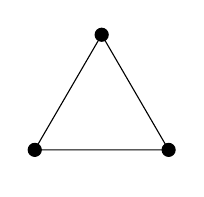
\begin{tikzpicture}[%
x={(1.7cm,0cm)},
y={(0cm,1.7cm)},
]

\coordinate (A) at (0,0); 
\coordinate (B) at (1,0) ;
\coordinate (C) at (0.5,0.86); 

%Ecken
\node[circle,scale=0.5,fill=black,draw=black](Ap) at (0,0){};
\node[circle,scale=0.5,fill=black,draw=black](Bp) at (1,0){};
\node[circle,scale=0.5,fill=black,draw=black](Cp) at (0.5,0.86){};

%Kanten
\draw[] (A)
-- (B)  node[midway, below]{}
-- (C)      node[midway, right]{}
-- (A)  node[midway, left]{};

\end{tikzpicture}
\subcaption{}
\end{minipage}
\hfill
 \begin{minipage}[t]{.2\textwidth}
   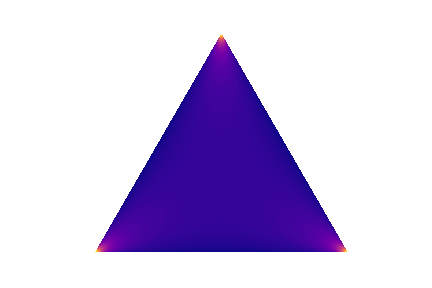
\includegraphics[width=\textwidth]{plots/notebooks/gs1.png}
\subcaption{}
\end{minipage}
\hfill
 \begin{minipage}[t]{.2\textwidth}
   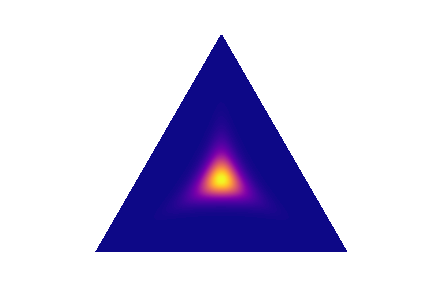
\includegraphics[width=\textwidth]{plots/notebooks/gs5.png}
\subcaption{}
\end{minipage}
\hfill
 \begin{minipage}[t]{.2\textwidth}
   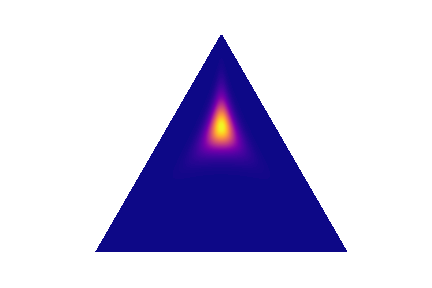
\includegraphics[width=\textwidth]{plots/notebooks/gs5_shift.png}
\subcaption{}
\end{minipage}

\caption{Пример распределения Gumbel-Softmax при различных значениях параметров: а)~$\lambda_{temp}\to0$, б)~$\lambda_{temp}=1, \mathbf{s}=[1,1,1]$, в)~$\lambda_{temp}=5, \mathbf{s}=[1,1,1]$, г)~$\lambda_{temp}=5, \mathbf{s}=[10,0.1,0.1].$}
\label{fig:gs}

\end{figure}


Заметим, что предлагаемое априорное распределение неоднозначно: одно и то же распределение  можно получить с различными значениями гиперпарамета $\mathbf{A}^{i,j}_k$ и структурного параметра $\gamma^{i,j}_k$. В качестве регуляризатора для матрицы $(\mathbf{A}^{i,j}_k)^{-1}$ предлагается использовать обратное гамма-распределение:
\[
    (\mathbf{A}^{i,j}_k)^{-1} \sim \text{inv-gamma}(\lambda_1,\lambda_2),
\]
где $\lambda_1,\lambda_2 \in \boldsymbol{\lambda}$ --- метапараметры оптимизации. 
Использование обратного гамма-распределения в качестве распределения гиперпараметров можно найти в~\cite{bishop,mackay}. В данной работе обратное распределение выступает как регуляризатор гиперпараметров.
Калибруя метапарамы   $\lambda_1,\lambda_2$ можно получить более сильную или более слабую регуляризацию~\cite{rvm}. Пример распределений $\text{inv-gamma}(\lambda_1,\lambda_2)$ для разных значений метапараметров $\lambda_1,\lambda_2$ изображен на Рис.~\ref{fig:inv-gamma}.

\begin{figure}
\centering
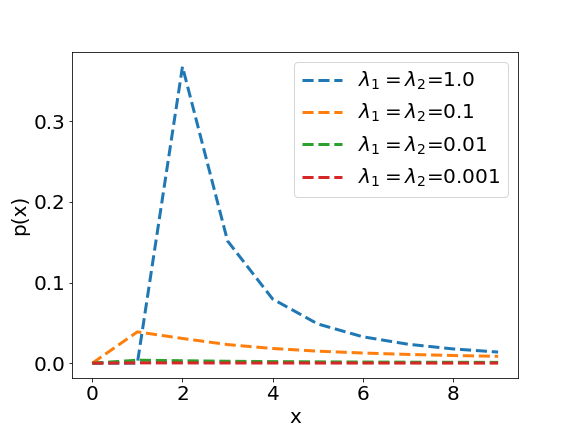
\includegraphics[width=0.6\textwidth]{plots/notebooks/invgamma.png}
\caption{Графики обратных гамма распределений для различных значений метапараметров.}
\label{fig:inv-gamma}
\end{figure}


Таким образом, предлагаемая вероятностная модель содержит следующие компоненты:
\begin{enumerate}
\item Параметры $\mathbf{w}$ модели, распределенные нормально.
\item Структура модели $\boldsymbol{\Gamma}$ распределены по распределению Gumbel-Softmax.
\item Гиперпараметры: $\mathbf{h} = [\text{diag}(\mathbf{A}), \mathbf{s}]$, где $\mathbf{A}$ --- конкатенация матриц $\mathbf{A}^{j,k}, (j,k) \in E,$ $\mathbf{s}$ --- конкатенация параметров Gumbel-Softmax распределений $\mathbf{s}^{j,k}, (j,k) \in E$, где $E$ --- множество ребер, соответствующих графу рассматриваемого параметрического семейства.
\item Метапараметры: $\boldsymbol{\lambda} = [\lambda_1, \lambda_2].$
\end{enumerate}

График вероятностной модели в формате плоских нотаций представлен на Рис.~\ref{fig:plate_prob}.
\begin{figure}
\centering
   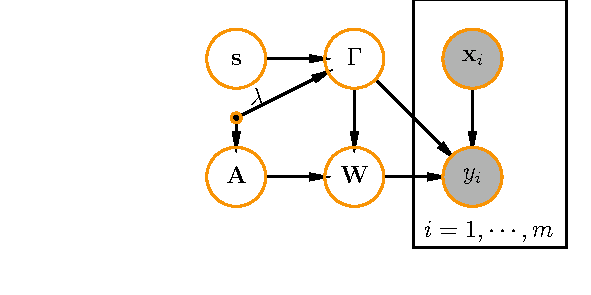
\includegraphics[width=0.5\textwidth]{plots/notebooks/simple_plate.pdf}
\caption{График предлагаемой вероятностной модели в формате плоских нотаций. Переменные обозначены белыми и серыми кругами, константы обозначены обведенными черными кругами. Наблюдаемые переменные обозначены серыми кругами.}
\label{fig:plate_prob}
\end{figure}

\section{Вариационная оценка для обоснованности вероятностной модели}
В качестве критерия выбора структуры модели предлагается использовать апостериорную вероятность гиперпараметров:
\begin{equation}
\label{eq:optimal_hyper}
    p(\mathbf{h}|\mathbf{y}, \mathbf{X}, \boldsymbol{\lambda}) \propto p(\mathbf{y}|\mathbf{X}, \mathbf{h}, \boldsymbol{\lambda}) p(\mathbf{h}|\boldsymbol{\lambda}) \to \max_{\mathbf{h} \in \mathbb{H}},
\end{equation}
где структура модели и параметры модели выбираются на основе полученных значений гиперпараметров:
\[
    \boldsymbol{\Gamma}^* = \argmax_{\boldsymbol{\Gamma} \in \amsmathbb{\Gamma}} p(\boldsymbol{\Gamma}|\mathbf{y}, \mathbf{X}, \mathbf{h}^*),
\]
\[
    \mathbf{w}^* = \argmax_{\mathbf{w} \in \mathbb{W}} p(\mathbf{w}|\mathbf{y}, \mathbf{X}, \boldsymbol{\Gamma}^*, \mathbf{h}^*),
\]
где $\mathbf{h}^*$ --- решение задачи оптимизации~\eqref{eq:optimal_hyper}.

Для вычисления обоснованности $$p(\mathbf{y}|\mathbf{X}, \mathbf{h}, \boldsymbol{\lambda}) = \iint_{\boldsymbol{\Gamma},\mathbf{w}}p(\mathbf{y}|\mathbf{X}, \mathbf{w}, \boldsymbol{\Gamma},\boldsymbol{\lambda})p(\mathbf{w}|\boldsymbol{\Gamma},\mathbf{h}, \boldsymbol{\lambda})p(\boldsymbol{\Gamma}|\mathbf{h}, \boldsymbol{\lambda})$$ из~\eqref{eq:optimal_hyper} предлагается использовать вариационную оценку обоснованности.

\begin{theorem}
Пусть $q = q_{\mathbf{w}}q_{\boldsymbol{\Gamma}}$ --- вариационное распределение c параметрами $\boldsymbol{\theta}$, аппроксимирующее апостериорное распределение структуры и параметров:
\[
    q (\mathbf{w},\boldsymbol{\Gamma}|\boldsymbol{\theta}) \approx p(\mathbf{w},\boldsymbol{\Gamma}|\mathbf{y}, \mathbf{X}, \mathbf{h}, \boldsymbol{\lambda}),
\]
\[
    q_{\mathbf{w}}(\mathbf{w}|\boldsymbol{\theta}_\mathbf{w},\boldsymbol{\Gamma}) \approx p(\mathbf{w}|\mathbf{y}, \mathbf{X},  \boldsymbol{\Gamma},\mathbf{h}, \boldsymbol{\lambda}),
\]
\[
    q_{\boldsymbol{\Gamma}}(\boldsymbol{\Gamma}|\boldsymbol{\theta}_{\boldsymbol{\Gamma}}) \approx p(\boldsymbol{\Gamma}|\mathbf{y}, \mathbf{X},  \mathbf{h}, \boldsymbol{\lambda}).
\]

Тогда справедлива следующая оценка:
\begin{equation}
\label{eq:full_elbo}
\text{log} p(\mathbf{y}|\mathbf{X}, \mathbf{h}, \boldsymbol{\lambda}) \geq
\end{equation}
\[
 \mathsf{E}_{\boldsymbol{\Gamma} \sim q_{\boldsymbol{\Gamma}}}\mathsf{E}_{\mathbf{w} \sim q_{\mathbf{w}}} \text{log}p(\mathbf{y}|\mathbf{w}, \boldsymbol{\Gamma}, \mathbf{X}) - D_\text{KL}\left(q_{\boldsymbol{\Gamma}}(\boldsymbol{\Gamma}|\boldsymbol{\theta}_{\boldsymbol{\Gamma}})|p(\boldsymbol{\Gamma}|\mathbf{h}, \boldsymbol{\lambda})\right) - D_\text{KL}\left(q_{\mathbf{w}}(\mathbf{w}|\boldsymbol{\theta}_\mathbf{w},\boldsymbol{\Gamma})|p(\mathbf{w}|\boldsymbol{\Gamma}, \mathbf{h})\right),
\]
где $D_\text{KL}\left(q_{\mathbf{w}}(\mathbf{w}|\boldsymbol{\theta}_\mathbf{w},\boldsymbol{\Gamma})|p(\mathbf{w}|\boldsymbol{\Gamma}, \mathbf{h})\right)$ вычисляется по формуле условной дивергенции~\cite{TODO}:
\[
D_\text{KL}\left(q_{\mathbf{w}}(\mathbf{w}|\boldsymbol{\theta}_\mathbf{w},\boldsymbol{\Gamma})|p(\mathbf{w}|\boldsymbol{\Gamma}, \mathbf{h})\right) = \mathsf{E}_{\boldsymbol{\Gamma} \sim q_{\boldsymbol{\Gamma}}} \mathsf{E}_{\mathbf{w} \sim q_{\mathbf{w}}} \frac{\text{log}q(\mathbf{w}|\boldsymbol{\Gamma})}{\text{log}p(\mathbf{w}|\mathbf{h},\boldsymbol{\Gamma})}.
\]
\end{theorem}

\begin{proof}
Используя неравенство Йенсена получим 
\[
\text{log} p(\mathbf{y}|\mathbf{X}, \mathbf{h}, \boldsymbol{\lambda}) \geq
\]
\[
   \mathsf{E}_{q} \text{log}p(\mathbf{y}|\mathbf{w}, \boldsymbol{\Gamma}, \mathbf{X}) - D_\text{KL}(q (\mathbf{w},\boldsymbol{\Gamma}|\boldsymbol{\theta})|p(\mathbf{w},\boldsymbol{\Gamma}|\mathbf{h})).
\]

Декомпозируем распределение $q$ по свойству условной дивергенции:
\[
D_\text{KL}(q (\mathbf{w},\boldsymbol{\Gamma}|\boldsymbol{\theta})|p(\mathbf{w},\boldsymbol{\Gamma}|\mathbf{h})) = D_\text{KL}\left(q_{\boldsymbol{\Gamma}}(\boldsymbol{\Gamma}|\boldsymbol{\theta}_{\boldsymbol{\Gamma}})|p(\boldsymbol{\Gamma}|\mathbf{h}, \boldsymbol{\lambda})\right) - D_\text{KL}\left(q_{\mathbf{w}}(\mathbf{w}|\boldsymbol{\theta}_\mathbf{w},\boldsymbol{\Gamma})|p(\mathbf{w}|\boldsymbol{\Gamma}, \mathbf{h})\right).    
\]
\end{proof}

В качестве вариационного распределения $q_{\mathbf{w}}$ предлагается использовать нормальное распределение, не зависящее от структуры модели $\boldsymbol{\Gamma}$:
\[
    q_{\mathbf{w}} = \mathcal{N}(\boldsymbol{\mu}, \mathbf{A}_q), 
\]
где $\mathbf{A}_q$ --- диагональная матрица с диагональю $\boldsymbol{\alpha}_q$.

В качестве вариационного распределения $q_{\boldsymbol{\Gamma}}$ предлагается использовать произведение распределений Gumbel-Softmax. конкатенацию параметров концентрации распределений обозначим как $\mathbf{s}_q$. Температуру вариационного распределения на структуре $\boldsymbol{\Gamma}$ обозначим как $\theta_\text{temp}$.

Вариационными параметрами распределения $q$ являются параметры распределений $q_{\mathbf{w}}, q_{\boldsymbol{\Gamma}}$:
\[
    \boldsymbol{\theta} = [\boldsymbol{\mu}, \boldsymbol{\sigma}^2_q, \mathbf{s}_q, \theta_\text{temp}], 
\]
где $ \mathbf{s}_q, \theta_\text{temp}$ --- параметры Gumbel-Softmax распределений.

График вероятностной вариационной модели в формате плоских нотаций представлен на Рис.~\ref{fig:plate_qprob}.
\begin{figure}
\centering
   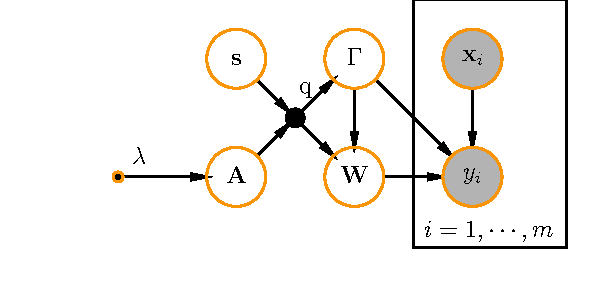
\includegraphics[width=0.5\textwidth]{plots/notebooks/plate.pdf}
\caption{График предлагаемой вероятностной вариационной модели в формате плоских нотаций. Переменные обозначены белыми и серыми кругами, константы обозначены обведенными черными кругами. Вариационное распределение обозначено черным кругом. Наблюдаемые переменные обозначены серыми кругами.}
\label{fig:plate_qprob}
\end{figure}


Для вычисления приближенного значения вариационной оценки обоснованности~\eqref{eq:full_elbo} предлагается использовать следующую формулу:
\[
    \sum_{r=1}^R \text{log}p(\mathbf{y}|\boldsymbol{\mu}+\boldsymbol{\alpha}_q \circ \hat{\epsilon}_r, \hat{\boldsymbol{\Gamma}}_r, \mathbf{X}) - \sum_{r=1}^R \left(\text{log}q_{\boldsymbol{\Gamma}}(\hat{\boldsymbol{\Gamma}}_r|\boldsymbol{\theta}_{\boldsymbol{\Gamma}})) - p(\hat{\boldsymbol{\Gamma}}|\mathbf{h},\boldsymbol{\lambda})\right) -
\]
\[ -\sum_{r=1}^R\frac{1}{2}\left( \hat{\boldsymbol{\Gamma}}_r^{-1}\text{tr}(\mathbf{A}_q\mathbf{A}^{-1}) + \boldsymbol{\mu}^{\mathsf{T}}\hat{\boldsymbol{\Gamma}}_r^{-1}\mathbf{A}^{-1}\boldsymbol{\mu} - |\mathbf{W}| + \text{log}\frac{|\boldsymbol{\Gamma}_r\mathbf{A}|}{|\mathbf{A})_q|}\right),
\]
где $r$ --- множество реализаций случайных величин, по котором вычисляется значения вариационной оценки обоснованности, $\hat{\epsilon}_r \sim \mathcal{N}(0,1),$
 $\hat{\boldsymbol{\Gamma}}_r$ --- реализация случайной величины, соответствующей структуре $\boldsymbol{\Gamma}$.

Для анализа сложности полученной модели введем понятие \textit{параметрической сложности}. 
\begin{defin}
Параметрической сложностью  $C_p(\boldsymbol{\theta})$ модели с вариационными параметрами $\boldsymbol{\theta}$ назовем минимальную дивергенцию между вариационным и априорным распределением:
\[
C_p(\boldsymbol{\theta}) = \min_{\mathbf{h} \in \mathbb{H}} \text{D}_\text{KL}\left(q(\mathbf{w}, \boldsymbol{\Gamma}|\boldsymbol{\theta})|p(\mathbf{w}, \boldsymbol{\Gamma}|\mathbf{h})\right).
\]
\end{defin}
Параметрическая сложность модели соответствует ожидаемой длине описания параметров модели при условии заданного параметрического априорного распределения~\cite{hinton_mdl}.

Одним из критериев удаления неинформативных параметров в вероятностных моделях является вариационная плотность~\cite{nips}: отношение вариационной плотности параметров в моде распределения к вариационной плотности параметра в нуле:
\[
    \frac{q_\mathbf{w}(\mu|\boldsymbol{\theta}_\mathbf{w})}{q(0)} = \text{exp}\left(-\frac{2\alpha_q^2}{\mu^2}\right),
\]
где $q_\mathbf{w}(w|\boldsymbol{\theta}_\mathbf{w}) \sim \mathcal{N}(\mu, \alpha_q).$

Обобщим понятие относительной вариационной плотности на случай произвольных распределений.
\begin{defin}
Относительной вариационной параметра  плотностью $w \in \mathbf{w}$  при условии структуры $\boldsymbol{\Gamma}$ и гиперпараметров $\mathbf{h}$ назовем отношение моды вариационного распределения параметра к моде априорного распределению параметра:
\[
    \rho(w|\boldsymbol{\Gamma}, \boldsymbol{\theta}_\mathbf{w}, \mathbf{h},\boldsymbol{\lambda}) = \frac{q\bigl(\text{mode}~q\left(w|\boldsymbol{\Gamma}, \boldsymbol{\theta}_\mathbf{w}\right)|\boldsymbol{\Gamma}\boldsymbol{\theta}_\mathbf{w}\bigr)}{q\bigl(\text{mode}~p\left({w}|\boldsymbol{\Gamma}, \mathbf{h},\boldsymbol{\lambda}\right)|\boldsymbol{\Gamma}\boldsymbol{\theta}_\mathbf{w}\bigr)},
\]
\[
    \boldsymbol{\rho}(\mathbf{w}|\boldsymbol{\Gamma}, \boldsymbol{\theta}_\mathbf{w}, \mathbf{h},\boldsymbol{\lambda}) = \prod_{w \in \mathbf{w}}\rho(w|\boldsymbol{\Gamma}, \boldsymbol{\theta}_\mathbf{w}, \mathbf{h},\boldsymbol{\lambda}).
\]

\end{defin}

Сформулируем и докажеми теорему о связи относительной плотности и параметрической сложности модели:
\begin{theorem}
Пусть вариационное распределение $q_\mathbf{w}$ и априорное распределение $p({w}|\boldsymbol{\Gamma}, \mathbf{h}))$ являются унимодальными со свойстом:
\[
    \text{mode}~q_\mathbf{w} = \mathsf{E}_{q_\mathbf{w}}w,\quad \text{mode}~p({w}|\boldsymbol{\Gamma}, \mathbf{h})) = \mathsf{E}_p({w}|\boldsymbol{\Gamma}, \mathbf{h}))~w.
\]
Пусть $\boldsymbol{\theta}_1,\boldsymbol{\theta}_2,\dots$ --- бесконечная по1следовательность векторов вариационных параметров, такая что $\lim_{i \to \infty}C_p(\boldsymbol{\theta}_i) = 0$, $\lim \sigma_q  \neq 0, \lim \theta_q \neq 0.$ 
С вариационной вероятностью $q_{\boldsymbol{\Gamma}}$ вариационная плотность данной последовательности стремится к единице:
\[
    \lim_{i \to \infty} \int_{\boldsymbol{\Gamma}} \boldsymbol{\rho}(\mathbf{w}|\boldsymbol{\Gamma}, \mathbf{h}_i)q(\boldsymbol{\Gamma})d\Gamma = 1, 
\]
где $\mathbf{h}_i = \argmin_{\mathbf{h} \in \mathbb{H}} \text{D}_\text{KL}\left(q(\mathbf{w}, \boldsymbol{\Gamma}|\boldsymbol{\theta})|p(\mathbf{w}, \boldsymbol{\Gamma}|\mathbf{h})\right)$. Пусть мода априорного распределения не зависит от гиперпарамтров.
\end{theorem}
\begin{proof}
Предел параметрической сложности перепишем как 
\[
    D_\text{KL}(q_\mathbf{w}|p|\boldsymbol{\gamma}) + D_\text{KL}(q_{\boldsymbol{\gamma}}|p).
\]
Т.к. параметрическая сложность состоит из двух неотрицательных слагаемых, то в пределе оба слагаемых достигают нуля.
Рассмотрим первое слагаемое:
\[
    D_\text{KL}(q_\mathbf{w}|p|\boldsymbol{\gamma}) = \mathsf{E}_q D_\text{KL}(q_\mathbf{w}|p|\boldsymbol{\gamma}).
\]
Отсюда и используя свойство теоремы о монотонной сходимости:
\[
    0 = \lim D_\text{KL}(q_\mathbf{w}|p|\boldsymbol{\gamma}) = \mathsf{E} \lim D_\text{KL}(q_\mathbf{w}|p|\boldsymbol{\gamma}).
\]
Поэтому для измеримого множества единичной меры дивергенция между априорным распределение и вариационным будет нулевой.
Рассмотрим разность предел разности мод двух распределений при $\Gamma$:
\[
    \lim (\text{mode} q -  \text{mode} p) = \lim \mathsf{E}_q \mathbf{w} - \mathsf{E}_p \mathbf{w} = \lim \int_\mathbf{w} \mathbf{w} (p-q) d\mathbf{w}.
\]
Т.к. $(p-q) \to 0$ почти наверно, то  %слабая сходимости
\[
    \lim \int_\mathbf{w} \mathbf{w} (p-q) d\mathbf{w} =  \int_\mathbf{w} \lim \mathbf{w} (p-q) d\mathbf{w} = 0.
\]
Отсюда разность мод для данных распределений в пределе равняется нулю.

Рассмотрим относительную плотность:
\[
    \frac{q}{q} = \lim = 1.
\]

\end{proof}
Теорема утверждает, что при устремлении параметрической сложности моделей к нулю, параметры модели станоятся неинформативными и подлежащими удалению. Заметим, что последовательность $q$ не обязана иметь предел. Примером такой последовательности может быть последовательность гауссовых распределений, чье среднее стремится к нулю.

\section{Обобщающая задача}
Рассмотрим основные критерии выбора вероятностных моделей.

\begin{enumerate}
\item Критерий максимального правдоподобия:
\[
    \text{log}p(\mathbf{y}|\mathbf{X}, \mathbf{w}) \to \max_{\mathbf{w} \in \mathbb{W}}.
\]

Метод заключается в максимизации правдоподобия обучающей выборки и подвержен переобучению.
Для использования данного метода в контексте вариационных распределений предлагается следующее обобщение:
\[
    L =  \mathsf{E}_q \text{log} \text{log}p(\mathbf{y}|\mathbf{X}, \mathbf{w}).
\]
Для данного метода нет оптимизируемых гиперпараметров. Для формального соответствия данной задачи задаче выбора положим $L=Q$.
Заметим, что частным случаем задачи является метод правдоподобия при выборе в качестве $q$ эмпирического распределения парамтетров и структуры.

\item Перебор структуры:
\[
    L =  Q = \mathsf{E}_q\text{log}p(\mathbf{y}, \mathbf{w}|\mathbf{X})[q_{\boldsymbol{\Gamma}} = p']
\]
где $p'$ --- некоторое распределение на структуре, выступающее в качестве метапараметра.


\item Метод максимальной апостериорной вероятности. 
\[
    \text{log}p(\mathbf{y},\mathbf{w}|\mathbf{X}, \mathbf{h} ) \to \max_{\mathbf{w} \in \mathbb{W}}.
\]
Аналогично предыдущему методу сформулируем вариационное обобщение данной задачи:
\[
    L = Q = \mathsf{E}_q \text{log} \text{log}p(\mathbf{y}|\mathbf{X}, \mathbf{w})+\text{log}p(\mathbf{w}|\boldsymbol{\lambda}) + \text{log}p(\boldsymbol{\gamma}|\mathbf{X}, \mathbf{w}).
\]
В рамках данной задачи оптимизации параметры априорных распределений $\mathbf{A}, \mathbf{s}$ выступают в качестве метапараметров, и поэтому не подлежат оптимизации.



\item Метод вариационной оценки обоснованности.
\[
    L = Q = \mathsf{E}_q \text{log}p(\mathbf{y}|\mathbf{X}, \mathbf{w}) - D_\text{KL}(q|p).
\]





\item Hold-out кросс-валидация.
\[
    L = \mathsf{E}_q \text{log}p(\mathbf{y}, \mathbf{w}|\mathbf{X}, \mathbf{h}),
\]
\[
    Q = \mathsf{E}_q \text{log}p(\mathbf{y}|\mathbf{X}, \mathbf{w}).
\]


\item Критерий Акаике:
\[
    \text{log}p(\mathbf{y}|\mathbf{X}, \mathbf{w}) - |\mathbb{W}|.
\]
Заметим,что в условия выбора модели на параметрическом множестве моделей данный критерий не имеет смысла, т.к. количество параметров для каждой модели одинаково. Прелагается следуюая переформулировка:
\[
    AIC_{\lambda} = \text{log}p(\mathbf{y}|\mathbf{X}, \mathbf{w}) - |\{w: C_p(w)<\lambda\}|.
\]

\item Информационный критерий Шварца:
\[
    \text{log}p(\mathbf{y}|\mathbf{X}, \mathbf{w}) - 0.5\text{log}(m)|\mathbb{W}|.
\]
Переформулируем данный критерий аналогично критерию AIC:
\[
    BIC_{\lambda} = \text{log}p(\mathbf{y}|\mathbf{X}, \mathbf{w}) - \text{log}(m)|\{w: C_p(w)<\lambda\}|.
\]

\end{enumerate}

Каждый из рассмотренных критерии удовлетворяет хотя бы одному из перечисленных свойтсв:
\begin{enumerate}
\item Модель, оптимизируемая согласно критерию, доставляет максимум правдоподобия выборки;
\item Модель, оптимизируемая согласно критерию, доставляет максимум оценки обоснованности;
\item Для моделей, доставляющих сопоставимые значения правдоподобия выборки, выбирается модель с меньшим количеством информативных параметров.
\item Критерий позволяет производить перебор структур для отбора наилучших модели.
\end{enumerate}

Формализуем рассмотренные критерии. Оптимизационную задачу, которая удовлетворяет всем перечисленным свойствам, будет называть \textit{обобщающей}.

\begin{defin}
Двухуровневую задачу оптимизации будем называть \textit{обобщающей} на области $U \subset \amsmathbb{\Theta} \times \mathbb{H} \times \amsmathbb{\Lambda}$, если она удовлетворяет следующим свойствам:
\begin{enumerate}
\item Для каждого значения гиперпараметров $\mathbf{h}$ оптимальное решение нижней задачи оптимизации $\boldsymbol{\theta}^{*}$ определено однозначно.
\item Свойство максимизации правдоподобия выборки: существует $\boldsymbol{\lambda} \in U_{\lambda}$ и  $K_1 \in \mathbb{R}_{+}$, такие что для любых векторов гиперпараметров $\mathbf{h}_1, \mathbf{h}_2 \in  U_{h}, Q(\mathbf{h}_1) - Q(\mathbf{h}_2) > K_1:$ матожидания правдоподбия выборок: $\mathsf{E}_q \text{log}~p(\mathbf{y}|\mathbf{X}, \boldsymbol{\theta}_1, \lambda_{\text{temp}}, \mathbf{f})>\text{log}\mathsf{E}_q ~p(\mathbf{y}|\mathbf{X}, \boldsymbol{\theta}_2, \lambda_{\text{temp}}, \mathbf{f})$.
\item Свойство минимизации параметрической сложности:  существует  $\boldsymbol{\lambda} \in U_{\lambda}$ и $K_2 \in \mathbb{R}_{+}$, такие что для любых векторов гиперпараметров $\mathbf{h}_1, \mathbf{h}_2 \in U_h, Q(\mathbf{h}_1) - Q(\mathbf{h}_2) > K_2$,  $\mathsf{E}_q \text{log}~p(\mathbf{y}|\boldsymbol{\theta}_1, \lambda_{\text{temp}}, \mathbf{f}) = \text{log}\mathsf{E}_q ~p(\mathbf{y}|\boldsymbol{\theta}_2, \lambda_{\text{temp}}, \mathbf{f})$, количество ненулевых параметров у первой модели меньше, чем у второй.
\item Свойства приближения оценки обоснованности: существует значение гиперпараметров $\boldsymbol{\lambda}$, такое что оптимизация задачи эквивалента оптимизации вариационной оценки обоснованности модели.
\item Свйоство перебора структур: существует константа $K_3$, такая что для любых двух векторов $\mathbf{h}_{1}, \mathbf{h}_2$ и соответствующих векторов $\boldsymbol{\theta}_1^{*},\boldsymbol{\theta}_2^{*}: D_\text{KL}(q_{\boldsymbol{\Gamma}_2}, q_{\boldsymbol{\Gamma}_1})>K_3, D_\text{KL}(q_{\boldsymbol{\Gamma}_1}, q_{\boldsymbol{\Gamma}_2})>K_3$:  существуют значения гиперпараметров $\boldsymbol{\lambda_1},\boldsymbol{\lambda_2}$, такие что  $Q(\mathbf{h}_1, \lambda_1) > Q(\mathbf{h}_2, \lambda_1), Q(\mathbf{h}_1, \lambda_1) < Q(\mathbf{h}_2, \lambda_2)$.

\item Свойсто нерперывности: $\mathbf{h}^{*}, \boldsymbol{\theta}^{*}$ непрерывны по метапараметрам.
\end{enumerate}
\end{defin}
Первое свойство говорит о том, что решение первого и второго уровня должны быть согласованы и определены однозначно.
Свойства 2-4 определяют возможные критерии оптимизации, которые должны приближаться обобщающей задачей.
Свойство 5 говорит о возможности перехода между различными структурами модели. Отметим, что данное условие крайне важно в условиях оптимизации моделей глубокого обучения, которые отличаются многоэкстремальностью.
Последнее свойство говорит о том, что обобщающая задача должна позволять производить переход между различными критериями выбора  параметров и структуры модели непрерывно.

\begin{theorem}Рассмотренные задачи не являются обобщающими.
\end{theorem}
\begin{proof}
TODO
\end{proof}

\begin{theorem}
Пусть задано непустое множество непрерывных по параметрам распределний на структуре $\mathbf{P}$. 
Пусть функции потерь и валидации $L,Q$ являются непрерывно-дифференцируемыми на некоторой области $U\subset \amsmathbb{\Theta} \times \mathbb{H} \times \amsmathbb{\Lambda}$, где параметры распределений $\mathbf{P} \in \amsmathbb{\Lambda}.$ 
Тогда следующая задача является обобщающей на $U$.
\begin{equation}
\tag{$Q^{*}$}
\label{eq:qopt}
\mathbf{h}^{*} = \argmax_{\mathbf{h}} Q = 
\end{equation}
\[
= {\lambda_\text{likelihood}^\text{Q}\mathsf{E}_{{q}^{*}} \text{log}~{p(\mathbf{y} | \mathbf{X}, \mathbf{w},\boldsymbol{\Gamma}, \mathbf{h}, \lambda_\text{temp}, \mathbf{f})}}
 -\]
\vspace{-0.3cm}
\[- {\lambda^\text{prior}_\text{Q}\text{D}_{KL}\bigl( q^{*}(\mathbf{w}, \boldsymbol{\Gamma}) || p(\mathbf{w}, \boldsymbol{\Gamma} |\mathbf{h}, \lambda_{\text{temp}},\mathbf{f}) \bigr)}  -\]
\vspace{-0.3cm}
\[
 - {\sum_{p' \in \mathbf{P}, \lambda \in \boldsymbol{\lambda}^\text{struct}_\text{Q}} \lambda\text{D}_{KL}(\boldsymbol{\Gamma} | p') + \text{log}p(\mathbf{h}|\mathbf{f})}, 
\]
где 
\begin{equation}
\tag{$L^{*}$}
{q}^{*} = \argmax_{q} L = 
{\mathsf{E}_q \text{log}~{p(\mathbf{y} | \mathbf{X}, \mathbf{w}, \boldsymbol{\Gamma}, \mathbf{h}, \lambda_{\text{temp}}, \mathbf{f})}}
\end{equation}
\vspace{-0.3cm}
\[- {\lambda^\text{prior}_\text{L}\text{D}_{KL}\bigl( q^{*}(\mathbf{w}, \boldsymbol{\Gamma}) || p(\mathbf{w}, \boldsymbol{\Gamma} |\mathbf{h}, \lambda_{\text{temp}},\mathbf{f}) \bigr)}.
\]
\end{theorem}
\begin{proof}
TODO
\end{proof}

Метапараметрами данной задачи являются коэффициенты $\lambda^\text{prior}_\text{Q}, \lambda^\text{prior}_\text{L}$, отвечающие за регуляризацию верхней и нижней задачи оптимизации, коэффициент $\lambda_\text{likelihood}^\text{Q}$ за максимизацию правдоподобия, а также параметры распрделений $\mathbf{P}$ и вектор коэффициентов перед ними $\boldsymbol{\lambda}^\text{struct}_\text{Q}$. 

В предельном случае, когда множество температура $\lambda_\text{temp}$ близка к нулю, а множество $\mathbf{P}$ состоит из распределений, близких к дискретным, и соответствующих всем возможным структурам, калибровка $\boldsymbol{\lambda}^\text{struct}_\text{Q}$ порождает последовательность задач оптимизаций, схожую с перебором структур. 

TODO

\textbf{Обобщающая задача: переформулировка через градиент}

\textbf{Обобщающая задача: адекватность задачи}

\textbf{Обобщающая задача: свойства коэффициентов}

\textbf{Решение задачи}

\textbf{Эксперимент: пример 1}

\textbf{Эксперимент: пример 2}









